\documentclass{article}
\usepackage[utf8]{inputenc}
\usepackage{amsmath}
\usepackage{amsfonts}
\usepackage{graphicx}
\usepackage{graphicx,wrapfig,lipsum}


\begin{document}

\title{PROBLEMS for NATIONAL MATHS AND PHYSICS OLYMPIAD}
\author{Prajit Adhikari}
\maketitle

\begin{enumerate}
    \item Prove that $5^n$ does not divide $(4n)!$ for any $k \in \mathbb{N}$.\\
    \textsc{Solution: }\\
    We have by Legendre's theorem,\\
    $$e_5(4n)= \bigg{\lfloor} \frac{4n}{5}  \bigg{\rfloor} + \bigg{\lfloor} \frac{4n}{5^2}  \bigg{\rfloor} + \bigg{\lfloor} \frac{4n}{5^3}  \bigg{\rfloor} +.....$$
    then, clearly, since $\bigg{\lfloor} n+k \bigg{\rfloor} =n$ for $k \in [0,1)$, we have,
    $$e_5(4n)< \frac{4n}{5}+ \frac{4n}{5^2}+.....= \frac{4n}{5}\bigg{(} 1+ \frac{1}{5} +\frac{1}{5^2} + ...... \bigg{)}$$
    $$e_5(4n)<\frac{4n}{5} \frac{1}{1-\frac{1}{5}} = n \implies e_5(4n) < n$$
    Hence, $5^k$ does not divide $(4n)!$.
    
    
    
    
    \item In any triangle $PQR$ prove that the reflection of orthocenter $H$ on any side $PQ, QR, RP$ lie on the circumcircle of $PQR$.
     \newline
    \textsc{Solution: }\\


    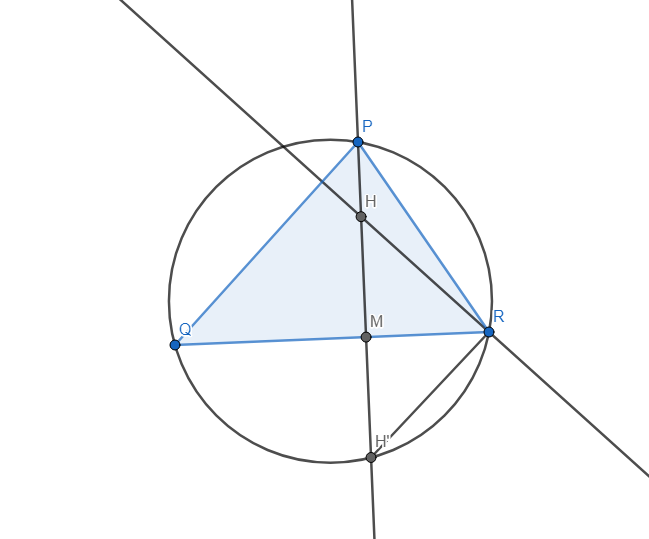
\includegraphics[width=5.5 cm]{Maths/geomtry.PNG}

    Let, $H'$ be the point of reflection of orthocenter through the side $QR$, and $M$ be the point on foot of altitude from $P$.
    Join $HR$ and $RH'$, then see that by $SAS$ axiom, 
    $$\Delta{RMH} \cong \Delta{RMH'} \implies \angle{RHM} = \angle{RH'M}$$
    
    Also, see that,
    $\angle{HPR} = 90^o - \angle{PRQ}, \angle{HRP} = 90^o - \angle{RPQ} $.
    Then, $\angle{RHM}=\angle{HPR}+\angle{HRP} =180^o -\angle{PRQ}-\angle{RPQ} $
    which is:
    $$ \angle{RH'M} = \angle{PQR} =\angle{RHM}$$
    By inscribed angle theorem, since $PR$ subtends same angle to $Q$ and $H'$, $H'$ lies on the circumcircle of $PQR$.\\
    
    \item In a small class of $12$ students, a random distinct two-digit number is assigned to each student. Call the set of groups "special" if the sum of assigned numbers of each students of the respective group is equal. Considering each group is distinct and a student can join two or more than two groups, prove that there must be a special set with at least $4$ groups.\newline
    \textsc{Solution: }\\
    See that, there are $2^{12}-1=4095$ subsets for the set of $12$ distinct two-digit numbers. However, see that the range of the sum of $12$ two digit number is just $\displaystyle{\sum_{i=88}^{99} i = 1122}$. Then, by pigeon hole principle there must be a set such that it has at least $\displaystyle{\bigg{\lceil} \frac{4095}{1122} \bigg{\rceil}=4}$ groups. And, we are done.
    \\
    P.S. If the participants, shows that $4095= 1122*3+729$, such that there is one group whose sum repeats at least thrice upto $1122*3$ subsets and then repeats again due to the remainder, he /she shall get full marks.
    
\end{enumerate}


\end{document}